
Talk about the problem setup, code blocks shown.

\begin{python}
"""
Set up and solve problem with identity map
"""
# import libraries
import bet.sample as sample
import bet.sampling.basicSampling as bsam
import numpy as np
import scipy.stats as sstats

# define input space parameters and model to instantiate sampler object
dimension = 2
numSamples = 100
I = np.eye(dimension)
def model(input_samples):
        return (I@input_samples.T).T
sampler = bsam.sampler(model)

# instantiate objects that hold input/output samples
input_set = bsam.random_sample_set('r', dimension, num_samples=numSamples)
disc = sampler.compute_QoI_and_create_discretization(input_set)

# define inverse problem
disc.set_initial(dist=sstats.uniform, loc=0, scale=1, gen=False)
disc.set_observed(dist=sstats.uniform, loc=0.4, scale=0.2)

disc_a = disc.copy()
# set analytical density (dimension is inferred)
disc_a.set_predicted(dist=sstats.uniform, loc=0, scale=1)

# create different sample sets with higher fidelity
disc_b = disc.copy()
disc_b.set_initial(num=int(1E3), gen=True)
# the line above removes the previous predicted distribution,
#     stored densities, probabilities, and volumes.
disc_c = disc.copy()
disc_c.set_initial(num=int(1E4), gen=True)
\end{python}

Note that there is no need to explictly call {\tt disc.compute\_pushforward()}, (or \pythoninline{disc.compute_predicted()}) since it is computed automatically if none have been previously constructed.
When \pythoninline{disc.updated_pdf()} is called, densities are evaluated at the initial set of $\nsamps$ random samples, and stored in \pythoninline{disc._input_sample_set._densities}.
However, the function \pythoninline{disc.predicted_pdf()} is capable of evaluating the solution at any new set of samples (provided a model is available/equipped to the discretization), something we leverage for plotting on a regular grid.

Once our four discretization objects \pythoninline{disc}, \pythoninline{disc_a}, \pythoninline{disc_b} and \pythoninline{disc_c} have been generated, we can use some utility plotting functions to compare the densities:

\begin{python}
"""
Plotting code to generate figures.
"""
# define plotting parameters
nbins = 50
xmn, xmx = 0.25, 0.75
ymn, ymx = 0.25, 0.75
xi, yi = np.mgrid[xmn:xmx:nbins*1j, ymn:ymx:nbins*1j]
# plotting functions call .get_updated(), which re-computes
# the pushforward distribution on a regular grid of samples
plot_2d_comparison(xi, yi, disc, disc_a, '$N=$100', 'Analytical')
plot_2d_comparison(xi, yi, disc_b, disc_c, '$N=$1,000', '$N=$10,000')
for d in [disc, disc_b, disc_c]:
    udpated_pdf_conditional_comparison(d, num=100, condition_on=0.5, label='approx')
\end{python}

\begin{figure}[ht]
\begin{minipage}{.975\textwidth}
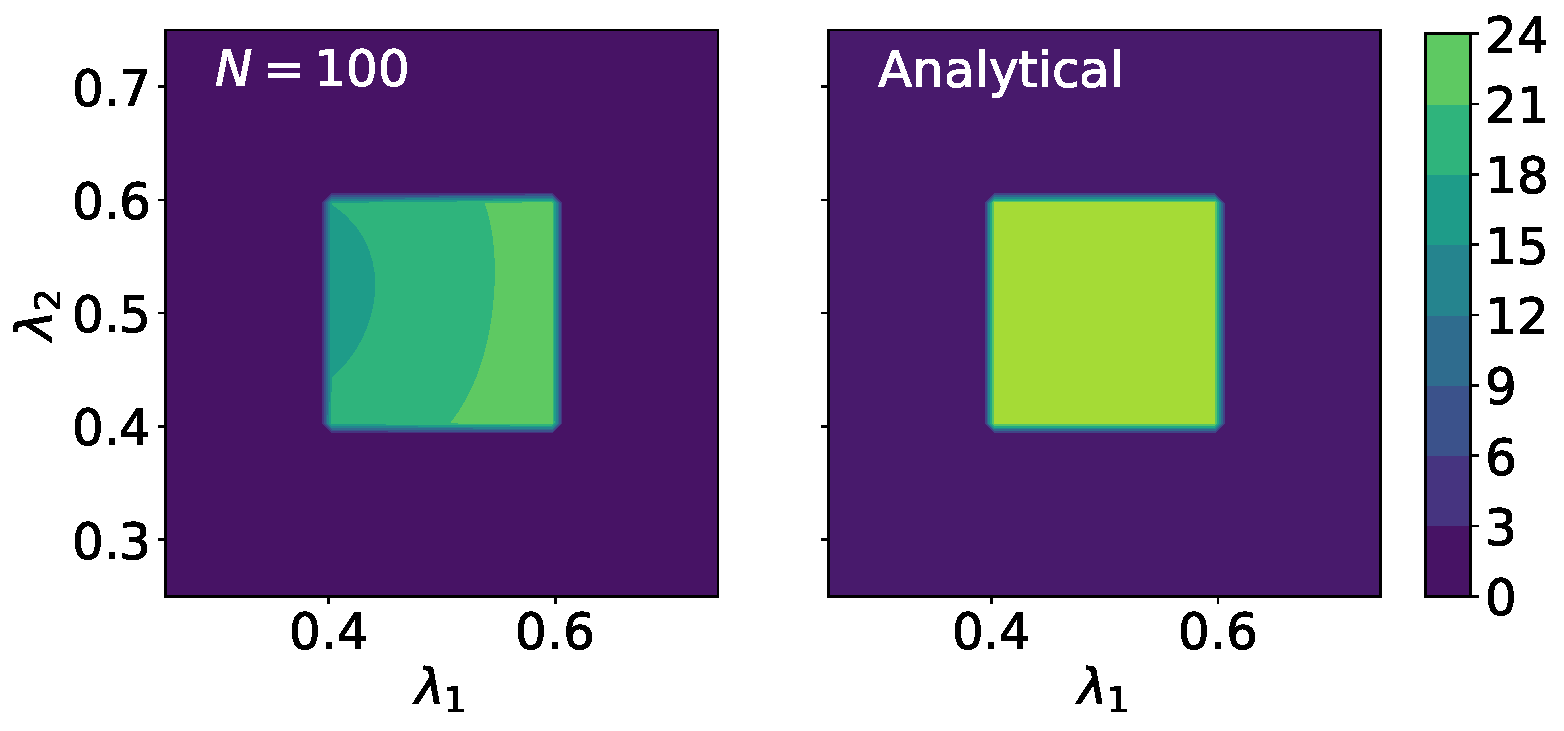
\includegraphics[width=\linewidth]{./examples/identity/samp/N100_N100-vs-Analytical_N100.pdf}
\end{minipage}
\caption{
(Left): $\nsamps=100$ were used to construct the predicted distribution $\predicted$.
(Right): By specifying an analytical $\predicted$, the effect of using $\nsamps$ to approximate a pushforward distribution disappears. The problem can be fully specified in BET without any random sampling.
}
\label{fig:ex:identity_sampling_exact}
\end{figure}

\begin{figure}[ht]
\begin{minipage}{.975\textwidth}
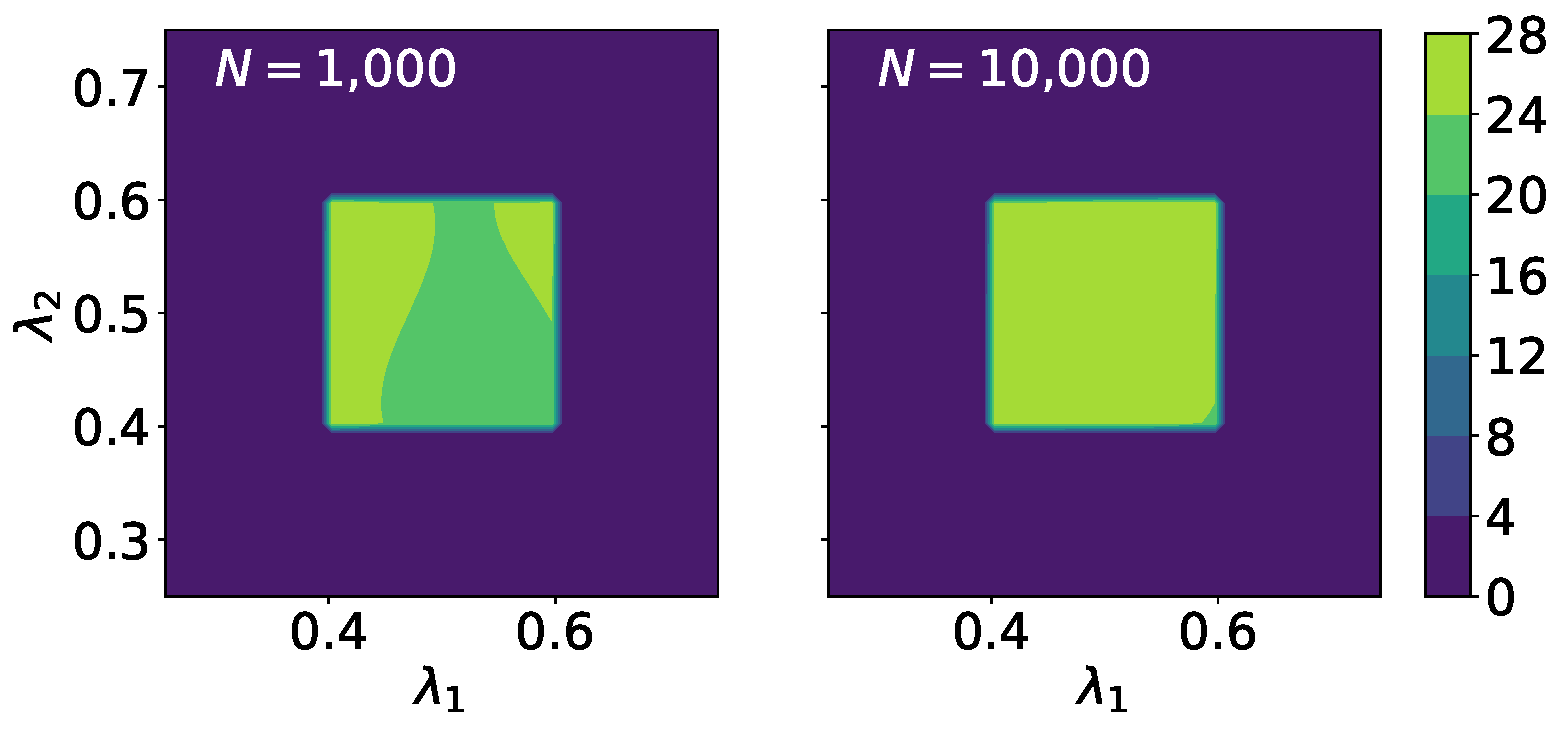
\includegraphics[width=\linewidth]{./examples/identity/samp/N1-000_N1000-vs-N10-000_N10000.pdf}
\end{minipage}
\caption{
$\nsamps=1,000$ (left) and $\nsamps=10,000$(right) were used to construct the predicted distribution $\predicted$.
There is no signficant error in estimating the support of the distribution, only the density approximation itself.
}
\label{fig:ex:identity_sampling_approx}
\end{figure}

\begin{figure}[ht]
\centering
	\begin{minipage}{.315\textwidth}
		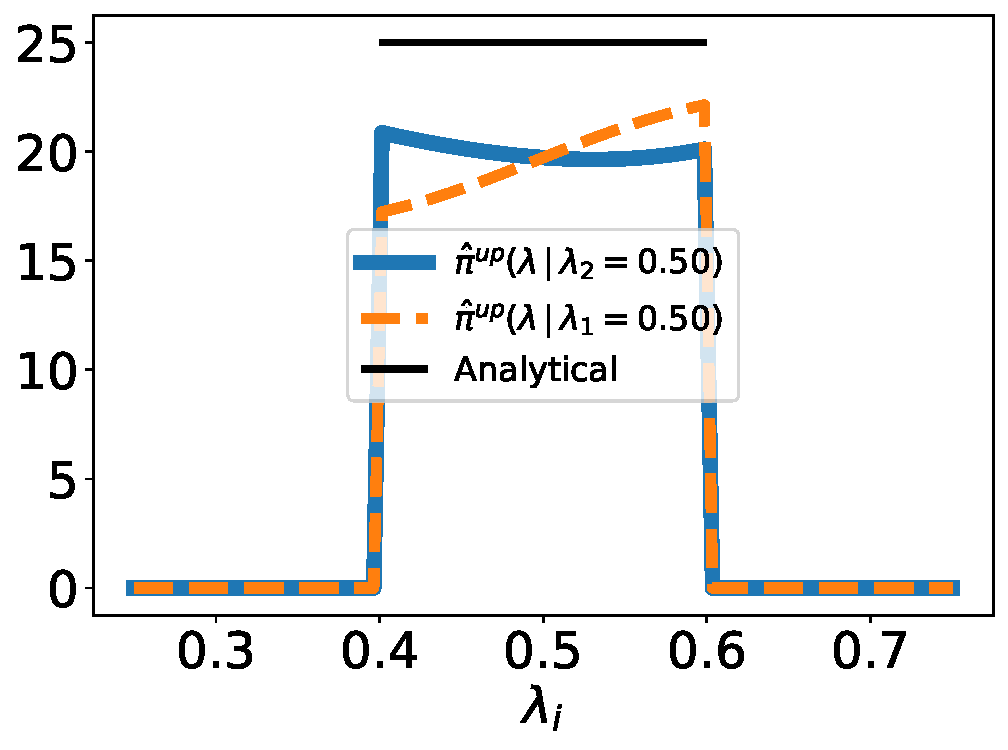
\includegraphics[width=\linewidth]{./examples/identity/samp/identity_1d_conditionals_50E-2_N100_approx.pdf}
	\end{minipage}
	\begin{minipage}{.315\textwidth}
		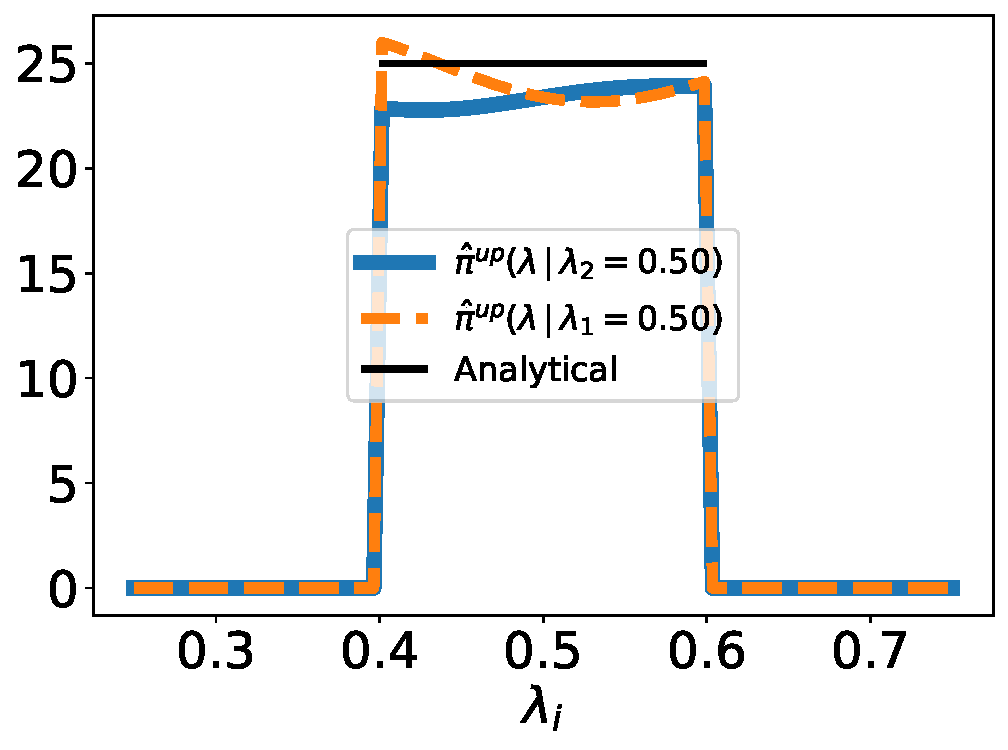
\includegraphics[width=\linewidth]{./examples/identity/samp/identity_1d_conditionals_50E-2_N1000_approx.pdf}
	\end{minipage}
  \begin{minipage}{.315\textwidth}
		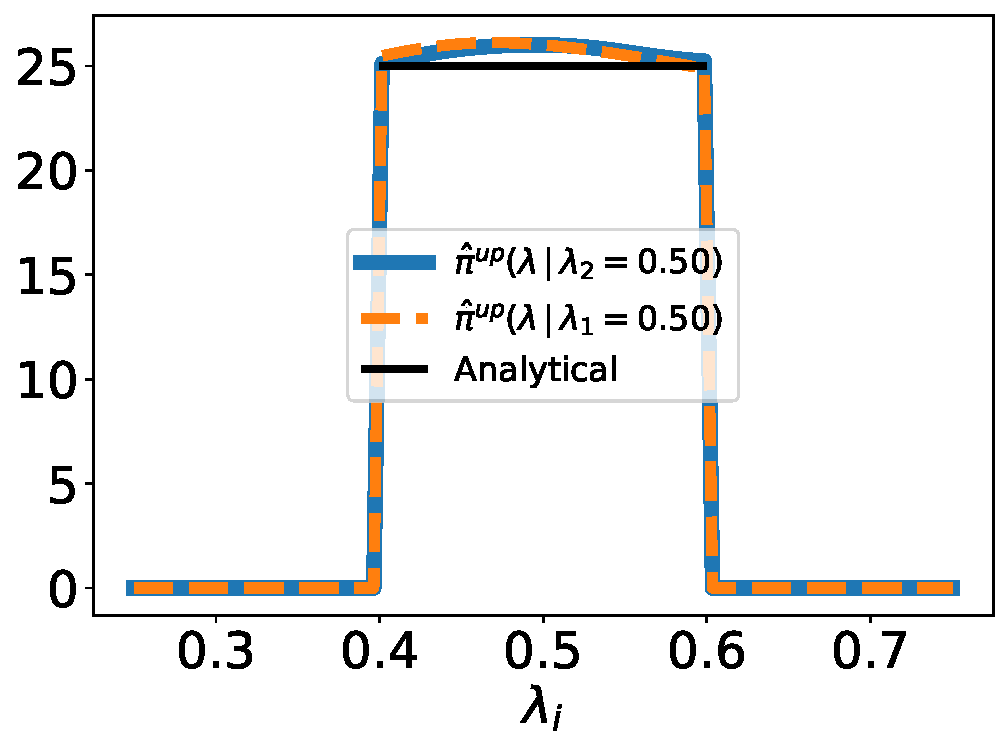
\includegraphics[width=\linewidth]{./examples/identity/samp/identity_1d_conditionals_50E-2_N10000_approx.pdf}
	\end{minipage}
\caption{
(Left to right, respectively): Conditionals passing through $(0.5, 0.5)$ for $\predicted$'s generated with $\nsamps=1E2, 1E3, \text{ and } 1E4$ random samples.
}
\label{fig:identity_sampling_conditionals}
\end{figure}
\FloatBarrier
